\section{Diseño}
\setlength{\parskip}{0.5cm}

En esta sección vamos a hablar del diseño de la aplicación. Volveremos un poco al diseño más clásico que es el diseño en cascada, pero seguiremos hablando en todo momento de metodología Kanban. 

\subsection{Volviendo al desarrollo en cascada}
Hemos dicho que la metodología de diseño que vamos a usar es Kanban, pero a mi personalmente me gusta siempre dar una serie de diagramas y de ideas procedentes del clásico desarrollo en cascada. Ya que las metodologías ágiles tienen unos entregables determinados y en ninguno de ellos aparecen los que yo voy a exponer a continuación, pero me parecen de una gran importancia y además expresan conceptos a nivel de arquitectura que a mi parecer deben de tener toda construcción de software. 

\subsubsection*{Elicitación de requisitos}

\textcolor{red}{Puede ser interesante meter una pequeña sección describiendo los requisitos funcionales y no funcionales de la aplicación, pero puede que sea introducir mucho la metodología en cascada}

\subsubsection*{Diagrama de clases de alto nivel}

\textcolor{red}{introducir un diagrama de clases aunque sea bastante simple? Puede estar interesante para mostrar los diferentes objetos que vamos a tener en representación a las tablas de la base de datos, pensar en ello}

\subsubsection*{Diagrama de casos de uso}

\textcolor{red}{lo equivalente al diagrama de casos de uso van a ser las diferntes US con el backlog, no se hasta que punto merece la pena ponerlo}

\subsubsection*{Diagrama de paquetes de alto nivel}

Uno de los diagramas que refleja muy bien la arquitectura que va a tener el sistema es el diagrama de paquetes, en el se suelen representar los diferentes paquetes y clases principales de las que se va a componer la aplicación. Podemos observar de un vistazo los principales patrones utilizados, así como las principales interacciones entre las diferentes partes que componen el sistema. 

El diagrama de paquetes, con los principales patrones que más se adecúan a la solución es el mostrado en la \textbf{Figura \ref{fig:diagramaPaquetes}}.

En esta arquitectura a alto nivel se puede apreciar el uso del modelo MVC, donde habrá clases que representen a la vista y accedan al modelo usando un controlador general de aplicación. Luego dicho controlador de aplicación es el que se encargará de interactuar con el resto de elementos y de proveer la información. 

Una de las partes más importantes de esta aplicación es el acceso a los datos, ya que vamos a estar interactuando de manera permanente contra una base de datos. Dichas peticiones tienen que ser eficientes y realizarse en el menor tiempo posible y de una manera sencilla. El patrón por el que he optado ha sido un patrón basado en objetos, es decir nosotros vamos a crear un ORM (Object Request Manager), que se va a encargar de atender las peticiones de información y va a devolver las filas de la base de datos en forma de objetos. 

Nuestra aplicación verá la base de datos como grandes listas de objetos. Cada de una base de datos será representada por un objeto diferente, con tantos atributos como columnas tenga dicha tabla. Cuando la aplicación necesite consultar una de esas filas, lo que hace nuestro ORM es devolver una lista con todas las filas de la base de datos en forma de lista de objetos. Entonces la aplicación se encarga de realizar la búsqueda dentro de esa lista. 

\begin{figure}[H]
    \centering
    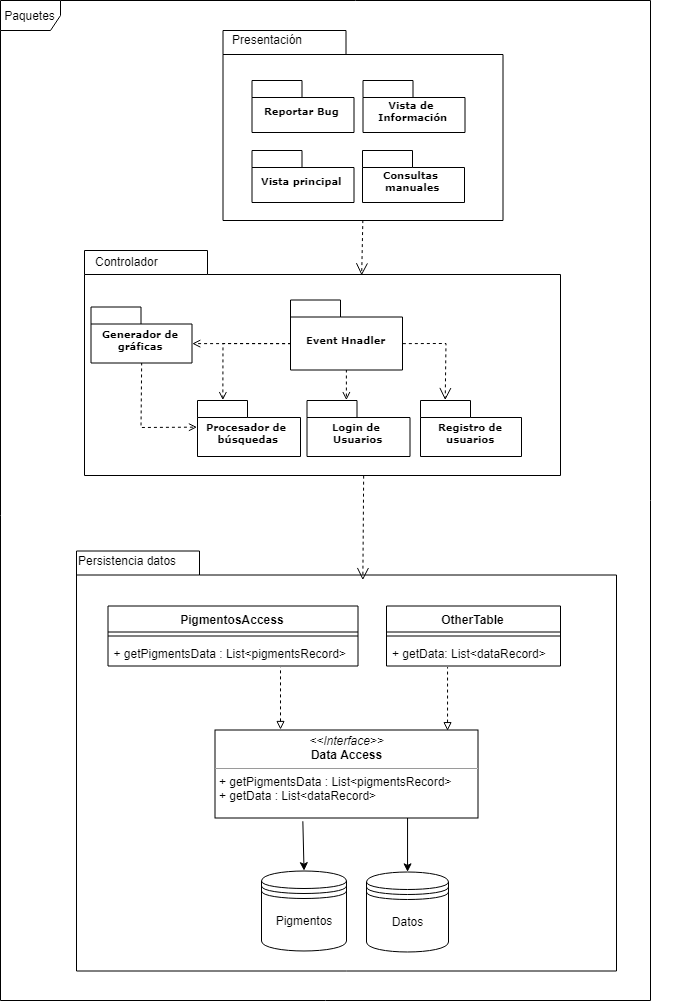
\includegraphics[scale=0.6]{imagenes/diseno/arquitecturaAltoNivel.png}
    \caption{Diagrama de Paquetes a alto nivel}
    \label{fig:diagramaPaquetes}
\end{figure}

\subsubsection*{Diagramas de secuencia de alto nivel}

En esta sección vamos a ilustrar como sería la interacción básica de los componentes de alto nivel de la aplicación. No buscamos una fuente detalla de los datos sino simplemente una aproximación a la solución que hemos planteado para que se entienda lo que hemos desarrollado en la aplicación, pero sin entrar a detalles de bajo nivel que pueden ofuscar la presentación. 

En este caso vamos a especificar un diagrama de secuencia para el supuesto de que el usuario quiere observar las propiedades químicas de un pigmento determinado. Esta secuencia de actividades la podemos ver reflejada a modo de ejemplo en el diagrama de la \textbf{Figura \ref{fig:diagramaSecuenciaVerPigmento}} 

\textcolor{red}{Hay que poner un OPT en el diagrama de secuencias, si tiene la información simplemente tiene que ir al objeto a buscarla, pero si no tiene que hacer otra consulta mediante el ORM para extraer la información de las tablas de la base de datos.}

\textcolor{red}{Igual hay que mirar de introducir algún diagrama de secuencia más, pero en principio este caso representa la funcioanldiad casi completa y básica de la aplicaicón}

\begin{figure}[H]
    \centering
    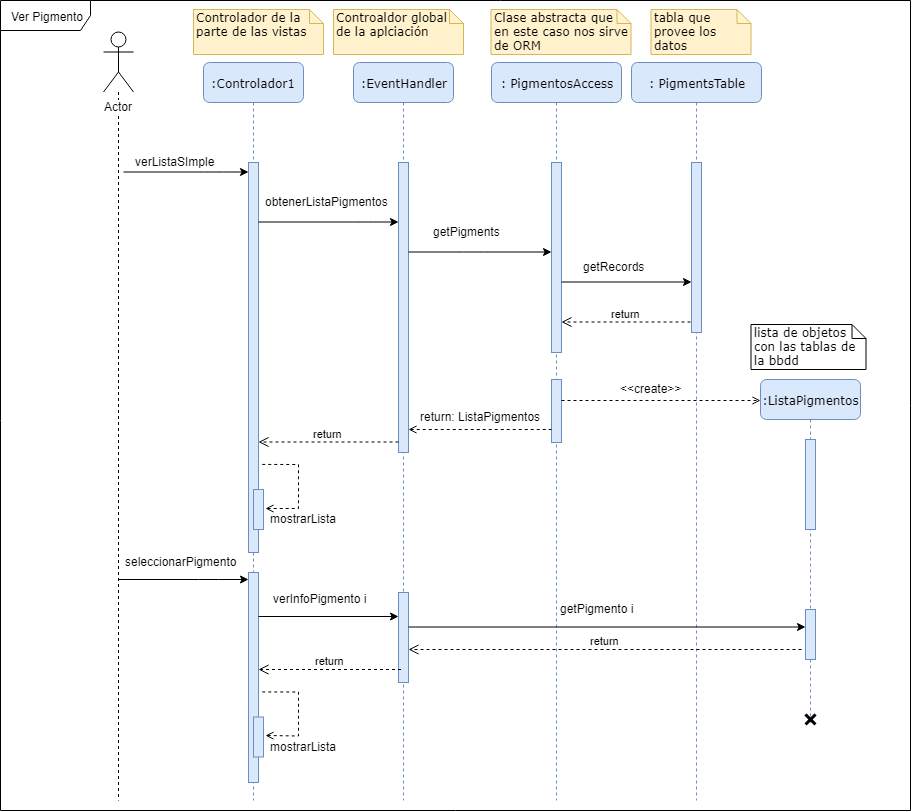
\includegraphics[scale=0.5]{imagenes/diseno/verInfoPigmentoSecuencia.png}
    \caption{Diagrama de secuencia de alto nivel para ver la información de un pigmento}
    \label{fig:diagramaSecuenciaVerPigmento}
\end{figure}

En este diagrama a de secuencias para uno de los casos más básicos, podemos observar como el actor interactúa con la aplicación y toca en el botón de ver todos los pigmentos, esta acción desencadena que el controlador del MVC se ponga en contacto con el controlador principal de la aplicación. Dicho controlador interactúa con el ORM que hemos dicho antes. Este ORM hace la consulta necesaria MySQL en la base de datos y le devuelve al controlador de aplicación una lista con todos los objetos representando las filas de la tabla que se haya consultado, en este caso la general de los pigmentos. El controlador de aplicación devuelve la información al controlador de la vista y presenta la información de una manera adecuada para el usuario. 

Ahora el usuario selecciona un pigmento en concreto, para ello el controlador de las vistas se pone en contacto con el controlador de la aplicación, el cuál no necesita interactuar con la base de datos porque ya tienes los datos disponibles. Buscamos el pigmento en cuestión, devolvemos la información al controlador de aplicación y este devuelve la información al controlador de las vistas. Hecho esto la el usuario tiene a su disposición la información que quería. 

Una vez que hemos presentado los principales diagramas e ideas en el formato tradicional, vamos a seguir con nuestra metodología inicial que es Kanban. 



\subsection{Definición de criterios}
En Kanban, antes de definir las historias de usuario, tenemos que definir brevemente alguno de los criterios que usaremos en dichas historias y que son muy importantes. 

Los más importantes que tenemos que definir son dos, los criterios de aceptación y los criterios de finalización.

\subsubsection{Definición de hecho}

La definición de hecho es una norma que se aplica a las Historias de Usuario, que desarrollaremos más adelante, pero para ello es necesario tener bien fijada esta definición con anterioridad. Normalmente esta definición es fijada de manera conjunta con el cliente final y el líder del equipo y muchas veces está presente el euqipo de desarrollo como tal para verificar las diferentes posibilidades, ya que nos permite:

\begin{itemize}
    \item \textbf{Tener un producto potencialmente entregable y usable} al finalizar cada iteración. En el caso de este proyecto no tenemos iteraciones como tal, pero si nosotros establecemos unas ciertas normas que tiene que cumplir cada una de las tareas que vamos a desarrollar, cuando nosotros finalicemos esas tareas podemos decir que están acabas y entregadas de manera adecuada y conforman el producto final perfectamente entrgeable. De esta forma el cliente, conforme tengamos tareas acabadas puede tomar decisiones de qué desarrollar en el futuro y qué no de manera clara y sencilla.
    
    \item \textbf{Establecer unos criterios de calidad}: define que entregables y mínimos de calidad se tienen que cumplir en todos los objetivos/requisitos que se van a ir aceptando conforme el proyecto vaya avanzando en el tiempo.
\end{itemize}

Ahora que sabemos lo que son y las posibilidades de la definición de hecho, pasamos a ver cuales serán nuestros criterios de hecho: 
\begin{enumerate}
    \item El trabajo de cada miembro del equipo ha sido revisado y aceptado por lo menos por una persona más del proyecto, que en este caso pueden ser tanto el tutor del proyecto como el profesor asociado.
    \item Todo el equipo considera que para cada objetivo/requisitos se cumplen sus criterios de aceptación al 100\%. 
    \item El requisito o tarea tiene que estar probado.
    \item Si el requisito lo permite, tiene que superar todas las pruebas unitarias que le hayan sido diseñadas. 
    \item Si el requisito lo permite, tiene que superar todas las pruebas de aceptación que le hayan sido diseñadas. 
    \item Si el requisito lo permite, tiene que superar todas las pruebas de regresión que le hayan sido diseñadas. 
    \item El requisito o tarea tiene que estar documentado.
    \item El requisito o tarea supera una calidad respecto a código del 80\%.
    \item El product owner ha validado y aceptado el objetivo/requisito.
\end{enumerate}

\subsubsection{Criterios de aceptación}

Mientras que los criterios de finalización tienden a ser criterios mas objetivos, medibles y triviales. Los criterios de aceptación dependen en gran medida del deseo e idea que el cliente tiene sobre el producto final. 

Los criterios de aceptación definen los requisitos del Product Owner sobre cómo debe comportarse la aplicación para que una determinada acción se pueda llevar a cabo, normalmente por parte de un usuario de la aplicación. Generalmente ayudan al equipo de desarrollo a responder a las preguntas: 
\begin{itemize}
    \item \textbf{¿He construido el producto correcto?}
    \item \textbf{¿He construido el producto correctamente?}
\end{itemize}

Los criterios de aceptación deben describir siempre un contexto, un evento y la respuesta o consecuencia esperada del sistema. La forma más utilizada para describir los criterios de aceptación es conocida como Given-When-Then, que veremos más adelante cuando mostremos las historias de usuario. 
Los criterios de aceptación son la clave de las historias de usuario, por lo tanto se tienen que cumplir todos los criterios de aceptación para dar una historia de usuario como terminada y correcta. 
El cumplimiento de los criterios de aceptación de las historias de usuario, a nivel de funcionalidad se verá de una manera muy clara cuando se presente la suite de pruebas asociadas a la aplicación. Como adelanto, dicha suite de pruebas se va a basar en un lenguaje llamado Gherkin en el que los escenarios de prueba se describen en un lenguaje de alto nivel basado en el Given-Then-When.

Habrá una asociación directa entre los criterios de aceptación de una historia de usuario y el test concreto que pruebe la funcionalidad de dicha historia de usuario. Todo esto lo podremos ver más en detalle en los capítulos posteriores, en concreto en el relacionado con las pruebas de la aplicación. 



\subsection{Épicas e historias de usuario}
A la hora de estructurar el trabajo que tenemos que hacer en un proyecto de gran magnitud, tenemos que tener en cuenta desde las actividades más ambiciosas hasta las mas detalladas. Por eso, existen diferentes estructuras de datos y formas de organización que nos ayuda a conseguir dicho objetivo. Como bien nos dice el \textit{Atlassian Agile Couch}, para conseguirlo nos podemos servir de los temas, iniciativas, épicas, historias de usuario y tareas. Podemos ver una descomposición visual de estos elementos en la \textbf{Figura \ref{fig:epicasHistorias}}

\begin{figure}[H]
    \centering
    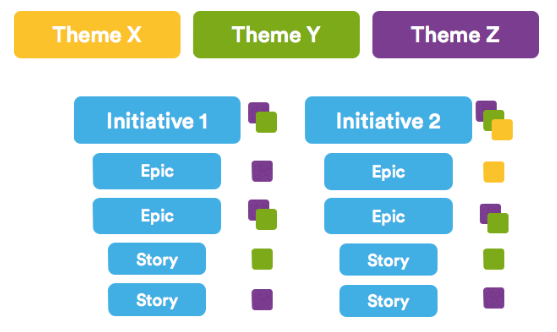
\includegraphics[scale=0.8]{imagenes/diseno/epicasHistorias.png}
    \caption{Relación entre épicas, historias y temas}
    \label{fig:epicasHistorias}
\end{figure}


A modo de resumen, cada una de las estructuras significa:
\begin{itemize}
    \item \textbf{Temas}: son grandes áreas de enfoque que abarcan a toda la organización.
    \item \textbf{Iniciativas}: son conjuntos de épicas que conducen hacia un objetivo común.
    \item \textbf{Épicas}: son grandes cantidades de trabajo que se pueden desglosar en un número de tareas más pequeñas, llamadas historias. 
    \item \textbf{Historias}: son breves requisitos o solicitudes escritas desde el punto de vista del usuario final. 
    \item \textbf{Tareas}: las tareas son actividades que hay que hacer para conseguir desarrollar las historias, no tienen porque estar escritas desde el punto de vista del cliente.  
\end{itemize}

En este proyecto por temas de magnitud, ya que es un proyecto pequeño, solo vamos a contar con historias, tareas y como mucho con unas cuantas épicas que nos van a venir bien a nivel de planificación y explicación del proyecto.

\subsubsection{Épicas}

Las épicas que nosotros vamos a presentar en nuestro proyecto son las siguientes: 
\begin{itemize}
    \item \textbf{Desarrollo}: en esta épica se incluirán las tareas relacionadas con las actividades de desarrollo.
    \item \textbf{Documentación}: se relacionarán tareas de documentación de las diferentes partes que componen el sistema, tanto documentación interna como documentación externa.
    \item \textbf{Configuración}: se añadirán las tareas relacionadas con la configuración de entornos o sistemas necesarios para la consecución de los objetivos del proyecto. 
    \item \textbf{Investigación}: puede que haya algunas tareas de investigación en ciertos puntos del proyecto, en esta épica habrá seguramente muy pocas tareas, pero también considero necesaria añadirla.
\end{itemize}

Cabe destacar que tanto las épicas del proyecto como las diferentes historias de usuario y tareas, las podemos 

\subsubsection{Historias de usuario}

Primero vamos a describir brevemente lo que son las épicas y las historias de usuario. Que son la base de la metodología que estamos siguiendo.

Las historias de usuario son la base trabajo de nuestro equipo de desarrollo. Para presentarlas hemos hecho una pequeña plantilla que muestra las características esenciales de una historia de usuario, y tiene los siguientes campos:
\begin{itemize}
    \item \textbf{Id}: cada una de las historias de usuario de nuestro proyecto va a tener un ID único que la identificará. Esto mejora la búsqueda de las mismas cuando hagamos referencias y siempre sepamos de que elemento estamos hablando. 
    
    \item \textbf{Prioridad Dev.}: número que seguirá la serie de Fibonacci (1, 3, 5, 8, 13, 21) que indicará la prioridad a la hora de desarrollar esa historia de usuario para los desarrolladores. Aclaramos que el 10 será la prioridad máxima y el 1 será la prioridad mínima. 
    
    \item \textbf{Valor}: número que seguirá la serie de Fibonacci (1, 3, 5, 8, 13, 21) que indicará la prioridad a la hora de desarrollar esa historia de usuario para el cliente final. Aclaramos que el 10 será la prioridad máxima y el 1 será la prioridad mínima. 
    
    \item \textbf{Estimación}: una ligera estimación del coste de implementación/finalización de esa Historia de Usuario. Podremos tener diferentes medidas, la mínima serán H (horas) y la máxima serán W (semanas). Ej.: 2H, 3D (días) o 1W. 
    
    \item \textbf{Asignado a}: desarrollador que tendrá asignado esa historia de usuario, aunque las tareas en las que se subdivida puedan estar asociadas a otros desarrolladores. 
    
    \item \textbf{Usuario}: el usuario al que va referida esta historia de usuario dentro de la aplicación final.
    
    \item \textbf{Descripción}: una breve descripción del objetivo que tiene que conseguir esa historia de usuario en concreto.
    
    \item \textbf{Dependencias}: las diferentes historias de usuario de las que depende la historia de usuario especificada. 
    
    \item \textbf{Criterios de aceptación}: los criterios que marcarán cuando la historia de usuario podrá considerarse cerrada y acabada. 
    
    \item \textbf{Épica relacionada}: se mostrará la épica con la que está asociada dicha tarea de usuario. \textcolor{red}{SI TODAS LAS HISOTIRAS VAN A ESTAR RELACIONADS CON UNA EPICA QUE SEA HISTORAS O DESARROLLO DE OALGO ASI, NO TIENE SENTIDO ESTE CAMPO}
    

\end{itemize}

Podemos ver una plantilla del formato que van a tener nuestras historias de usuario en la siguiente \textbf{Figura \ref{fig:formatoHistoria}}

\begin{figure}[H]
\centering
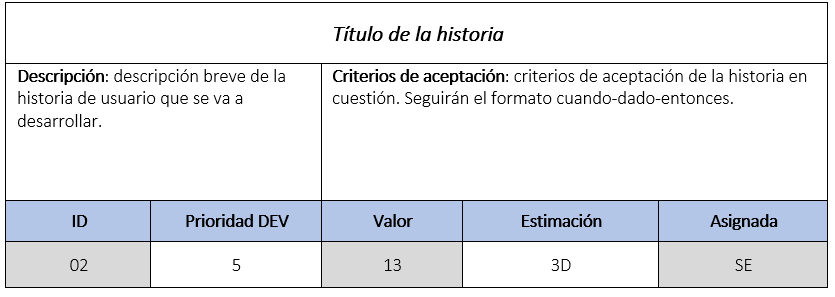
\includegraphics[scale=0.6]{imagenes/diseno/formatoHistoria.png}
\caption{Formato que seguirán las historias de usuario}
\label{fig:formatoHistoria}
\end{figure}

Una vez que hemos definido el formato de nuestras historias de usuario, los criterios que van a tener y todas las partes de las que van a constar, podemos pasar a mostrar todas las que tenemos. 

\subsection{Backlog}
El backlog es una de las herramientas mas importantes cuando hablamos de desarrollo de proyectos bajo el marco de las metodologías ágiles. El backlog es una estructura de datos, normalmente una lista que contiene todas las historias de usuario y tareas que se van desarrollando en la aplicación. El bakclog normalmente se ordena de manera inicial por la prioridad que el cliente asigna, pero sin embargo es común que dentro de esa prioridad del cliente se reordene también por la prioridad que los desarrolladores consideran necesaria. Esto se debe a que el cliente puede considerar muy necesaria una de las historias, pero sin embargo es muy fácil de desarrollar en comparación a otras tareas que pueden conllevar una carga de desarrollo mayor. 

A continuación voy a mostrar el backlog con todas las historias de usuario que consideramos necesarias. Este backlog estará replicado en taiga.io. Además en el backlog de la aplicación se podrán observar las diferentes épicas, y tareas relacionadas con cada una de las diferentes historias, que también estarán en el backlog. 

\begin{figure}[H]
    \centering
    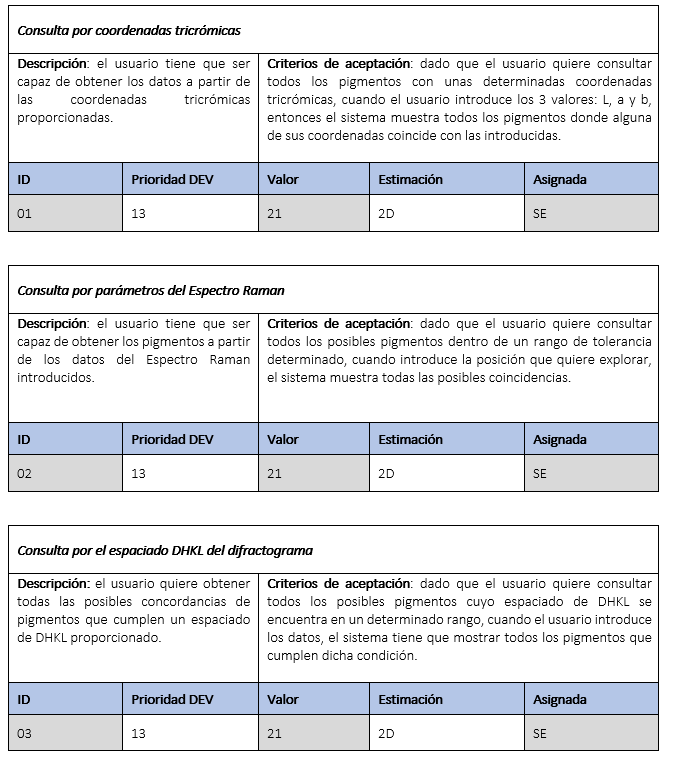
\includegraphics[scale=0.8]{imagenes/diseno/us13.png}
    \label{fig:us13}
\end{figure}

\begin{figure}[H]
    \centering
    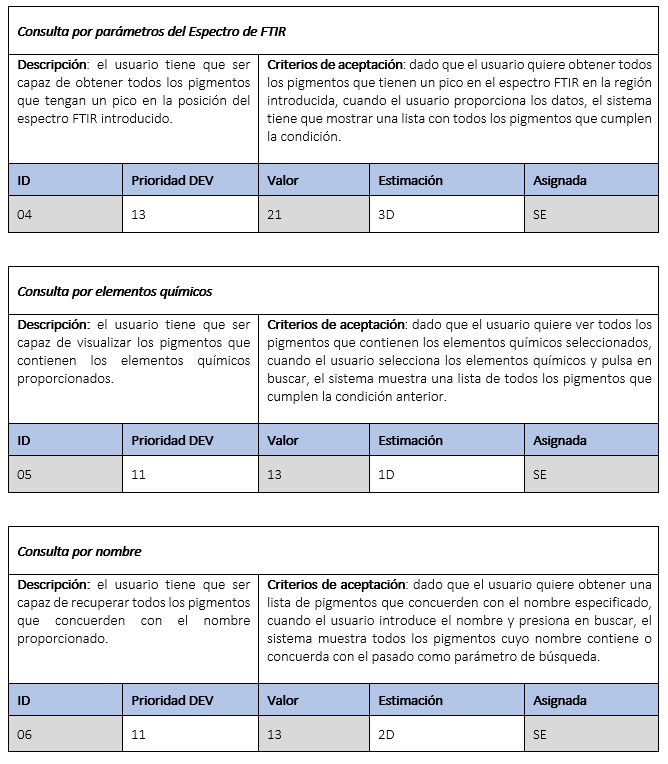
\includegraphics[scale=0.8]{imagenes/diseno/us46.png}
    \label{fig:us46}
\end{figure}

\begin{figure}[H]
    \centering
    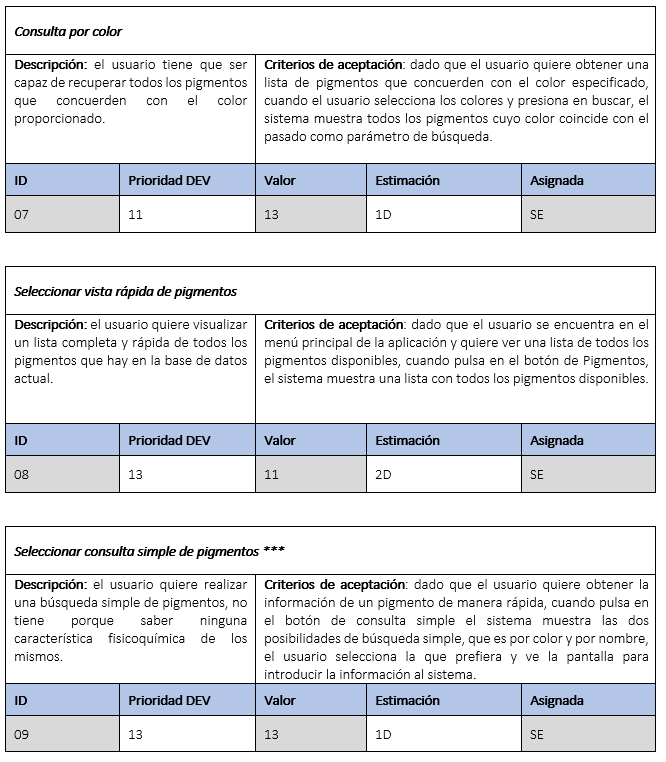
\includegraphics[scale=0.8]{imagenes/diseno/us79.png}
    \label{fig:us79}
\end{figure}

\begin{figure}[H]
    \centering
    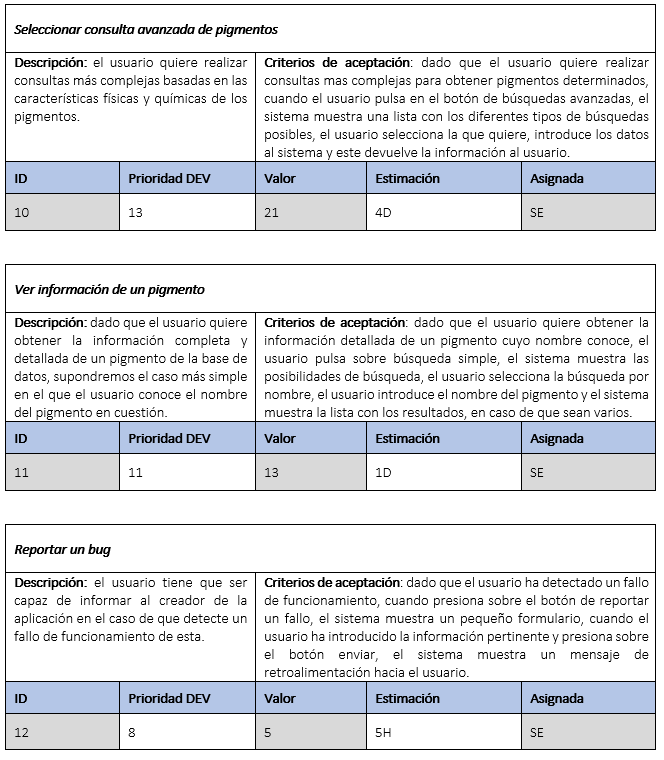
\includegraphics[scale=0.8]{imagenes/diseno/us1012.png}
    \label{fig:us1012}
\end{figure}

\begin{figure}[H]
    \centering
    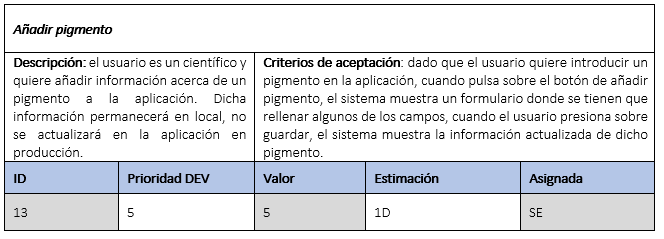
\includegraphics[scale=0.8]{imagenes/diseno/usTrece.png}
    \label{fig:usTrece}
\end{figure}

Ahora que ya tenemos el backlog ordenado, sabemos las tareas que tenemos que desarrollar, como hay que hacerlo y en que orden, podemos pasar a empezar a desarrollar la aplicación y pensar en cosas de más bajo nivel. También podemos observar, que estas historias de usuario tiene diferentes dependencias entre ellas, como es esperable en el desarrollo de una aplicación, por ejemplo podemos completar la parte de las consultas avanzadas si no tenemos el desarrollo de la interfaz principal. 

La precedencia de tareas la podemos observar en la \textbf{Figura \ref{fig:precedenciaTareas}}

\begin{figure}[H]
    \centering
    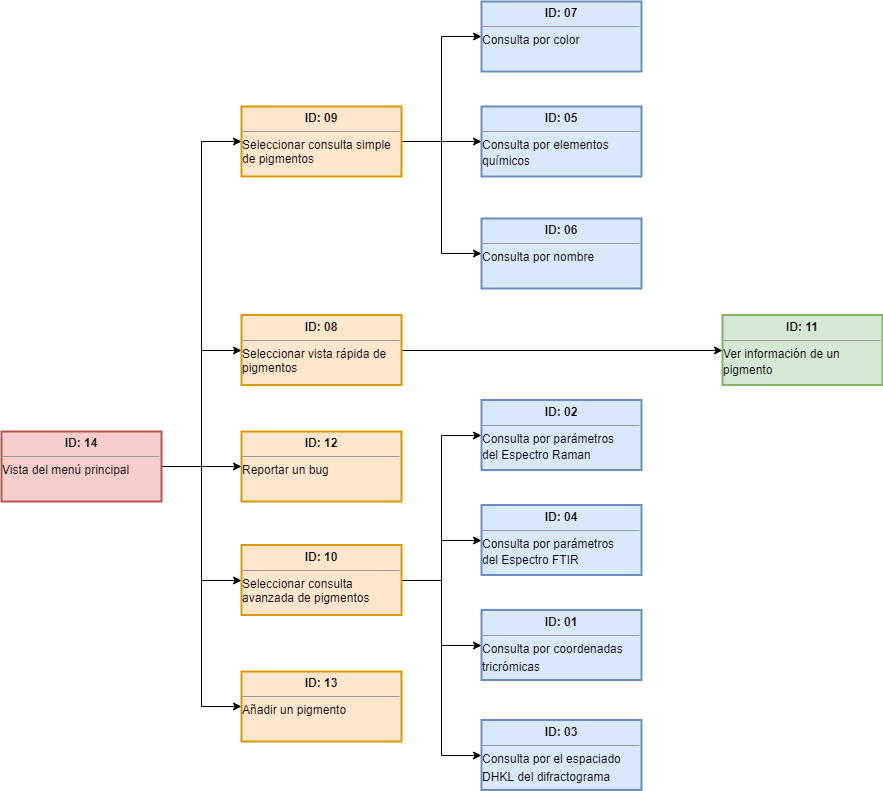
\includegraphics[scale=0.5]{imagenes/diseno/precedenciasTareas.png}
    \caption{Diagrama de precedencia de las principales tareas}
    \label{fig:precedenciaTareas}
\end{figure}

Muchas de las tareas, como la ID:07, ID:05 o ID:02 desembocan también en la ID:11, pero no están relacionadas porque no es estrictamente necesario que todas ellas estén terminadas para poder empezar la 11, la única que si que tiene que estar necesariamente terminada para poder empezar con la ID:11 es la ID:08. 



\subsection{Bocetos iniciales}
Ahora que tenemos planificadas la gran mayoría de tareas principales y a más alto nivel, vamos a empezar con el desarrollo como tal de la aplicación. En esta sección presentaremos el logo de la app junto con el nombre y los diseños de las principales interfaces. 

\subsubsection{Logo de la aplicación y nombre}

Una de las primeras cosas en las que pensamos cuando escuchamos aplicación móvil es en el nombre y el logo de las grandes aplicaciones. En la época actual los logos tienen a ser minimalistas, simples y con colores pastel y suaves. Así mismo los nombres de las aplicaciones tienden a ser cortos, ya que los dispositivos móviles suelen tener un tamaño reducido y no se pueden meter frases largas. 

\subsubsection*{Logo}

Los dos diseños iniciales para el logo de la aplicación fueron los siguientes: 

\begin{multicols}{2}
    \begin{figure}[H]
        \centering
        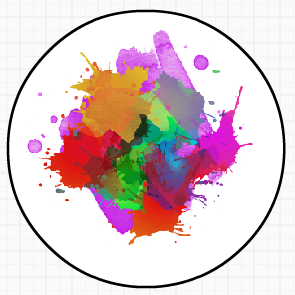
\includegraphics[scale=0.8]{imagenes/diseno/logo1.png}
        \caption{Diseño 1 del logo de la aplicación}
        \label{fig:logo1}
    \end{figure}
    
    \begin{figure}[H]
        \centering
        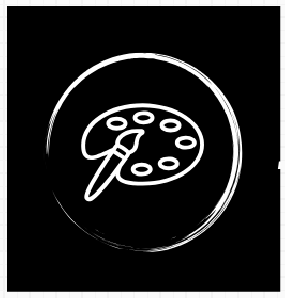
\includegraphics[scale=0.8]{imagenes/diseno/logo2.png}
        \caption{Diseño 1 del logo de la aplicación}
        \label{fig:logo2}
    \end{figure}
\end{multicols}

Pero después de una reunión con el cliente final, se llego a la conclusión de que el logo debería de ir mas por el estilo de la paleta:

\begin{figure}[H]
    \centering
    
\includegraphics[scale=0.3]{imagenes/diseno/logo3.png}
    \caption{Diseño final del logo de la aplicación}
    \label{fig:logo3}
\end{figure}

\subsubsection*{Nombre}

En la sección anterior ya hemos dejado ver cual iba a ser el nombre de la aplicación. Una de las ideas iniciales era:
\begin{itemize}
    \item \textbf{PigemtsDB}: pero ni al cliente ni al tutor del TFG les convencía esta opción, ya que al contener la acortación DB, procedente de Data Base incluía unas connotaciones un poco más técnicas.
\end{itemize}

Al final se ha dejado como \textbf{Pigment Studio} ya que tiene un significado ligeramente más general y no restringe a ningún tipo de colectivos. 

Es un nombre corto y que haces una buena referencia a lo que el usuario se va a encontrar cuando abra la aplicaicón, que no es más que un estudio bastante avanzado y claro de los diferentes pigmentos que tenemos en el mundo. 

\subsubsection{Diseño de las primeras interfaces}

Una de las partes más críticas cuando estamos desarrollando aplicaciones que va a utilizar el usuario final es la interfaz que van a tener que usar. Va a ser una pantalla contra la que el usuario va a interactuar bastante a menudo, por lo tanto tiene que ser cómoda, clara y sencilla. Algunas de las normas que tienen que tener el diseño de interfaces para que el usuario tenga una buena experiencia (UX) las podemos encontrar en la siguiente lista \textcolor{red}{buscar en la bibliografía de IPC algo sobre el diseño de interfaces de usuario y citar un par de libros}: 
\begin{itemize}
   \item 
\end{itemize}

Las principales interfaces que vamos a encontrar en nuestro sistema son las siguientes, junto con una descripción de lo que harán. 

\subsubsection*{Menú Principal}

En el menú principal de la aplicación podremos encontrar las diferentes opciones que nos presenta para explotar la base de datos de la manera más adecuada. Entre ellos los botones que nos podemos encontrar (recordar que solo son bocetos):
\begin{itemize}
    \item \textbf{Pigmentos}: en esta sección encontraremos una lista con todos los pigmentos que tenemos en la base de datos con algunas características en miniatura.
    \item \textbf{Consulta Simple}: nos permitirá realizar las principales consultas, que son por color y por el elemento químico principal del pigmento en cuestión. 
    \item \textbf{Consulta Avanzada}: nos permitirá realizar búsquedas más avanzadas, como por las coordenadas tricrómicas de un pigmento o por determinadas características de las gráficas de los mismos.
    \item \textbf{Gráficas}: mostrará al usuario una lista de las diferentes gráficas que se disponen de cada pigmento.
    \item \textbf{Añadir Pigmento}: el usuario podrá añadir un nuevo pigmento a la base de datos, en el caso de que se disponga de los datos suficientes para hacerlo. 
\end{itemize}

Podemos ver la vista del menú principal en la \textbf{Figura \ref{fig:menuPrincipal}}

\newpage
\begin{multicols}{2}
    \begin{figure}[H]
    \centering
    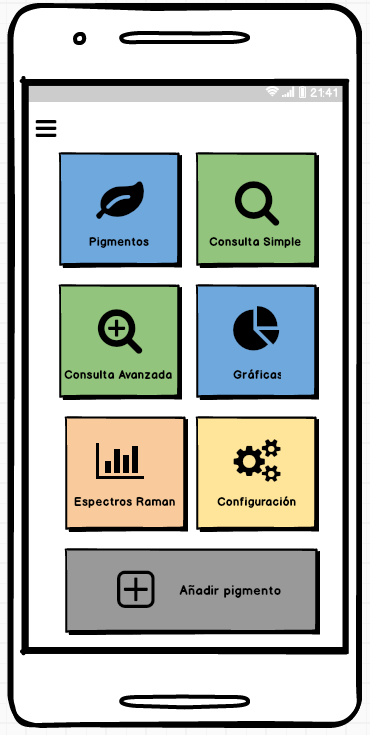
\includegraphics[scale=0.6]{imagenes/diseno/main.png}
    \caption{Menú principal de la aplicación}
    \label{fig:menuPrincipal}
    \end{figure}
    
    \begin{figure}[H]
    \centering
    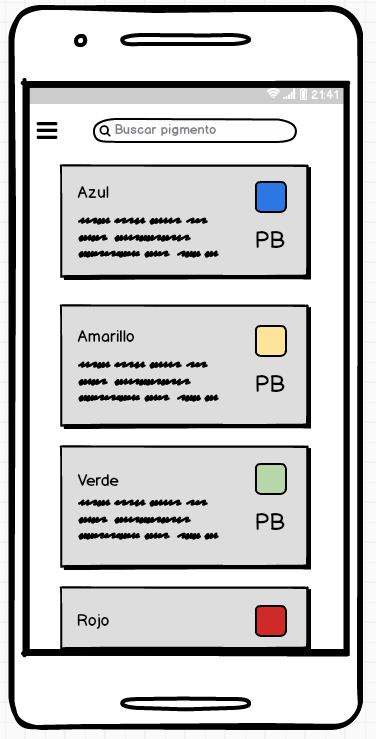
\includegraphics[scale=0.6]{imagenes/diseno/lista.png}
    \caption{Lista principal con todos los pigmentos del sistema}
    \label{fig:listaPigmentos}
    \end{figure}
\end{multicols}

\subsubsection*{Vista rápida de pigmentos}

Si el usuario pulsa sobre el botón de pigmentos, entonces lo que se va a encontrar es una sencilla lista con todos los pigmentos que se encuentran disponibles en el sistema. La entrada de cada pigmento constará del nombre del mismo, un color aproximado, para que se le haga mas visual al usuario, junto con una breve descripción y en miniatura el elemento químico principal que compone dicho pigmento. Podemos observar dicho menú en la \textbf{Figura \ref{fig:listaPigmentos}}. En esta vista el usuario puede buscar por nombre un determinado pigmento, puede conseguir esto introduciendo el nombre del mismo en la barra superior que tenemos en el menú.

\subsubsection*{Información de los pigmentos}

Una vez que en la pantalla que hemos presentado anteriormente, el usuario pulsa sobre uno de los pigmentos, el sistema muestra toda la información detalla del mismo según la \textbf{Figura \ref{fig:infoPigmentos}}

\newpage
\begin{multicols}{2}
    \begin{figure}[H]
    \centering
    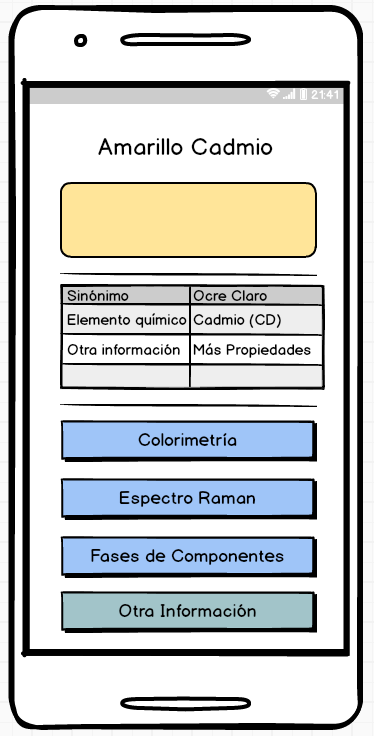
\includegraphics[scale=0.6]{imagenes/diseno/inforPigmento.png}
    \caption{Información de los pigmentos}
    \label{fig:infoPigmentos}
    \end{figure}
    
    \begin{figure}[H]
    \centering
    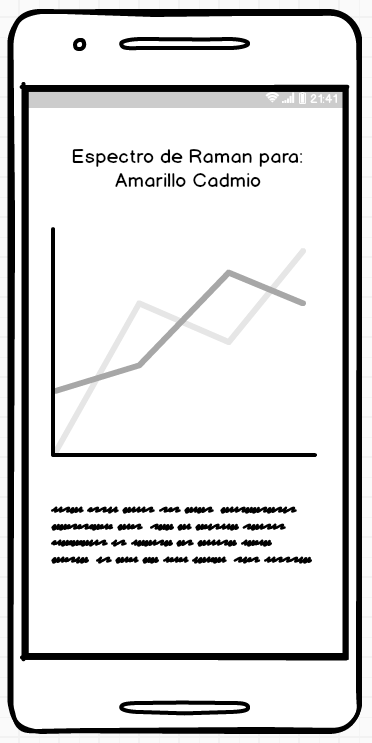
\includegraphics[scale=0.6]{imagenes/diseno/infoGraficas.png}
    \caption{Información gráficas de pigmentos}
    \label{fig:infoGraficas}
    \end{figure}
\end{multicols}

\subsubsection*{Consulta Simple - Opción 1}

Volviendo al menú principal, si el usuario pulsa sobre el botón de consulta simple entonces se le muestran las diferentes opciones, que en este caso solo son 3, una es la búsqueda por color, otra la búsqueda por un elemento químico y la tercera es la opción que tendríamos en el menú principal de verlos todos. Además una vez que el usuario pulsa sobre una de las dos opciones, el sistema le muestra los diferentes formularios para ejecutar la búsqueda. 

En esta sección tenemos que presentar dos bocetos diferentes, que son los que se habían pensado en el principio, y luego se darán más detalles para decir con cual nos hemos decantado. 

Podemos ver los primeros bocetos en las Figuras siguientes:

\newpage
\begin{multicols}{3}
    \begin{figure}[H]
    \centering
    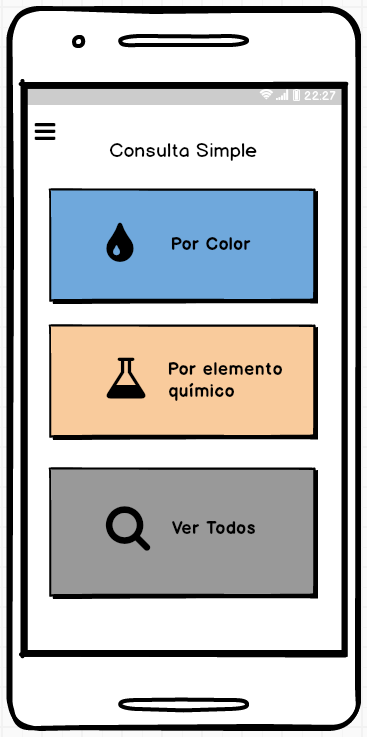
\includegraphics[scale=0.5]{imagenes/diseno/simpleQuery.png}
    \caption{Menú para hacer una consulta simple}
    \label{fig:consultaSimple}
    \end{figure}
    
    \begin{figure}[H]
    \centering
    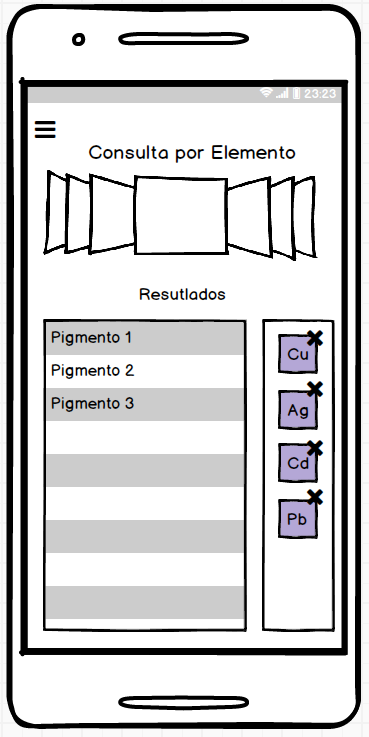
\includegraphics[scale=0.5]{imagenes/diseno/elementos1.png}
    \caption{Menú de selección de colores}
    \label{fig:consultaColores}
    \end{figure}
    
    \begin{figure}[H]
    \centering
    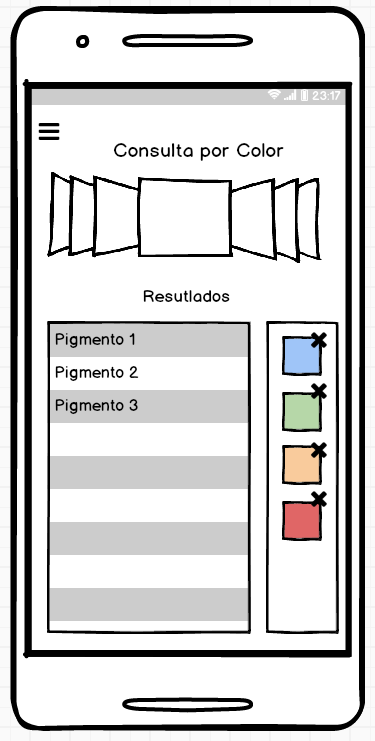
\includegraphics[scale=0.5]{imagenes/diseno/color1.png}
    \caption{Menú de selección de elementos}
    \label{fig:consultaElementos}
    \end{figure}
\end{multicols}

En la \textbf{Figura \ref{fig:consultaSimple}} podemos ver el menú principal que hemos descrito anteriormente, donde el usuario elije el tipo de búsqueda que quiere realizar. Mientras que en la \textbf{Figura \ref{fig:consultaColores}} podemos ver la selección de colores y en la \textbf{Figura \ref{fig:consultaElementos}} podemos ver como sería la pantalla de selección de elementos. 

La ventaja que tienen estas interfaces es que puedes un solo diseño de la vista de la aplicación para dos funcionalidades diferentes. Además es más dinámica ya que evita tener que pulsar tantos botones como las opciones que mostraremos a continuación. El usuario simplemente desliza en busca de los colores o elementos que quiere, va pulsando sobre ellos, dichos elementos se van añadiendo a la lista vertical de la derecha, y la lista de resultados se va actualizando automáticamente en función de los filtros introducidos. 

\subsubsection*{Consulta Simple - Opción 2}

Sin embargo en las \textbf{Figuras \ref{fig:consultaColores1}} y \textbf{Figuras \ref{fig:consultaElementos1}} podemos ver como era otra de las ideas iniciales para estas consultas.

\newpage
\begin{multicols}{2}
    \begin{figure}[H]
    \centering
    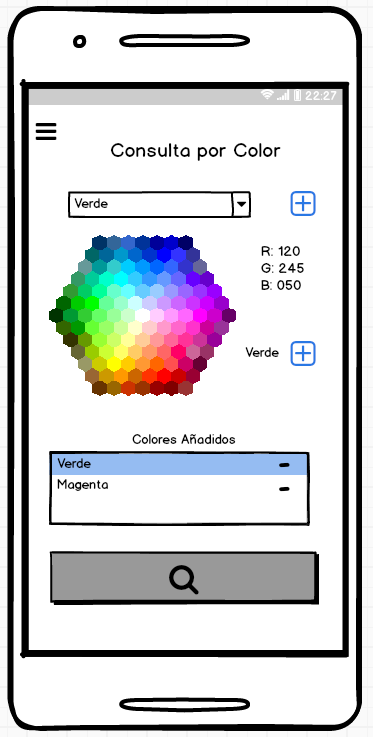
\includegraphics[scale=0.6]{imagenes/diseno/porColor.png}
    \caption{Menú de selección de colores}
    \label{fig:consultaColores1}
    \end{figure}
    
    \begin{figure}[H]
    \centering
    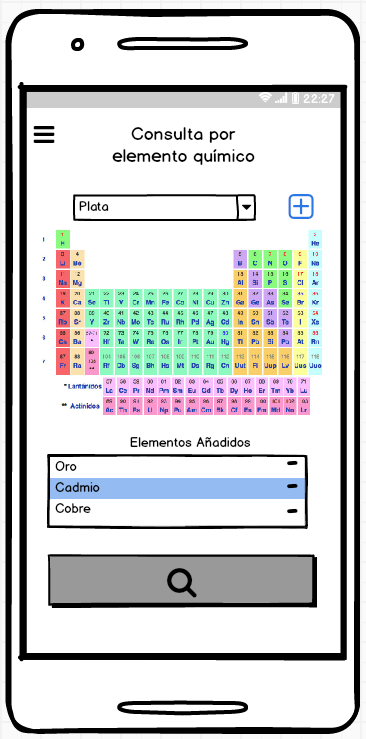
\includegraphics[scale=0.6]{imagenes/diseno/porElemento.png}
    \caption{Menú de selección de elementos}
    \label{fig:consultaElementos1}
    \end{figure}
\end{multicols}

Las desventajas que podemos encontrar al diseñar esta interfaz son varias. Primero es menos dinámica que la opción anterior ya que el usuario tiene que hacer más pulsaciones en la pantalla para obtener el mismo resultado, además de que tiene más pantallas intermedias, ya que se tienen que mostrar los resultados en una vista diferente. Otra de las desventajas desde el punto de vista de desarrollo es que requieren funcionalidades diferentes, en una tendríamos que añadir un selector de color e introducir cosas más específicas de este elemento mientras que la otra opción tendríamos que ingeniarnos un selector de elementos químicos, lo cual puede ser complicado. La opción anterior unifica estas opciones, ya que saca los colores y los elementos de una base de datos y solo tiene que cargar la información para que el usuario la elija como filtro de la búsqueda. 

Recordamos que las figuras anteriormente presentadas son solo bocetos de la aplicación. La idea es que la aplicación final quede de manera aproximada a como se ha mostrado, pero por problemas de desarrollo, tiempo u otras causas es posible que los resultados finales se vean afectados o no sean completamente fieles a los presentados en las figuras anteriores. 

\subsubsection*{Reportar Bug}

Esta pantalla no tiene mucha importancia a nivel de funcionalidad, pero si que la considero bastante importante a nivel de peticiones de cambio futuras y cuyo objetivo es mejorar la aplicación el tiempo. 

Los reportes de fallos o bugs de la aplicación, que sea reportados por los usuarios serán almacenados en un servidor central que gestionará una base de datos de fallos y bugs. Esta información se mandará de manera completamente anónima por la red, y no se almacenará ningún posible dato del usuario. 

La pantalla que tengo pensada para implementar esta funcionalidad la podemos observar en la \textbf{Figura \ref{fig:bugreport}}

\begin{figure}[H]
\centering
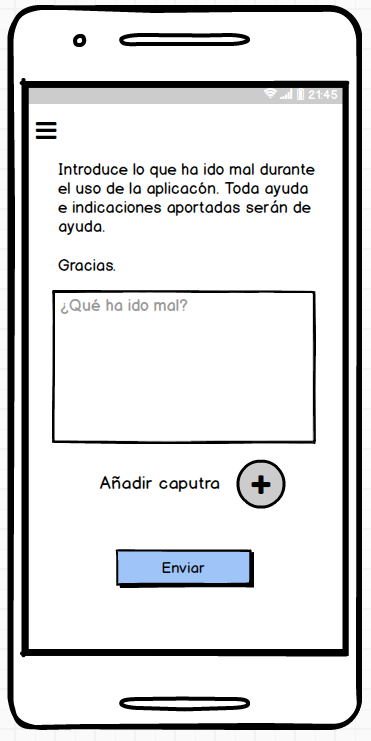
\includegraphics[scale=0.6]{imagenes/diseno/bugreport.png}
\caption{Menú de reporte de fallos}
\label{fig:bugreport}
\end{figure}


\subsection{Sistema de Integración continua}
El sistema de integración continua ha sido ligeramente descrito en los capítulos anteriores (\textbf{Sección \ref{sec:jenkins}}) cuando hablábamos de la tecnología que íbamos a utilizar, que en este caso es Jenkins. 

Cabe destacar que los sistemas de integración continua y entrega continua son más relevantes en equipos de desarrollo grandes con muchos servicios diferentes. Por ejemplo si el equipo de desarrollo hace un despliegue de una nueva versión de los servicios en un entorno determinado, entonces se pasan una serie de pruebas automáticas para ver que nadie ha roto nada, etc. Sin embargo ya que la magnitud de nuestro proyecto es pequeña, esta parte tampoco tiene demasiada importancia, aunque intentaré reflejarla tal cual lo hacen las empresas en la actualidad. 

Si nos basamos en la teoría fundamental de la integración continua y del proceso de pruebas, las pruebas del sistema deberían de empezar en paralelo con el desarrollo de la aplicación, mientras que las pruebas unitarias de los diferentes métodos se diseñan antes de la implementación de dichos métodos [\textcolor{red}{REFERENCIA EL ISTQB}]. 

En este caso lo que voy a hacer es desarrollar la interfaces más principales de la aplicación. Una vez desarrolladas esas interfaces se diseñarán los casos de prueba más simples para dichas pantallas, los cuales se introducirán en Jenkins y desde entonces se pasarán de manera automática cada vez que se haga un push en el sistema de control de versiones. 

Cuando tengamos que desarrollar algún algoritmo o método, la idea es que se desarrollen algunas pruebas unitarias mínimas para probar la funcionalidad de dicha parte del método. Estas pruebas también se añadirán en trabajos diferentes a la parte de Jenkins para que se pasen de manera automática.

Entraremos más en detalle en el funcionamiento y test exactos del sistema de integración continua cuando hablemos de la calidad que queremos del software y desarrollemos las pruebas de la aplicación. 


